%\title{LaTeX Portrait Poster Template}
%%%%%%%%%%%%%%%%%%%%%%%%%%%%%%%%%%%%%%%%%
% a0poster Portrait Poster
% LaTeX Template
% Version 1.0 (22/06/13)
%
% The a0poster class was created by:
% Gerlinde Kettl and Matthias Weiser (tex@kettl.de)
% 
% This template has been downloaded from:
% http://www.LaTeXTemplates.com
%
% License:
% CC BY-NC-SA 3.0 (http://creativecommons.org/licenses/by-nc-sa/3.0/)
%
%%%%%%%%%%%%%%%%%%%%%%%%%%%%%%%%%%%%%%%%%

%----------------------------------------------------------------------------------------
%	PACKAGES AND OTHER DOCUMENT CONFIGURATIONS
%----------------------------------------------------------------------------------------

\documentclass[a0,portrait]{a0poster}

\usepackage{multicol} % This is so we can have multiple columns of text side-by-side
\columnsep=100pt % This is the amount of white space between the columns in the poster
\columnseprule=3pt % This is the thickness of the black line between the columns in the poster

\usepackage[svgnames]{xcolor} % Specify colors by their 'svgnames', for a full list of all colors available see here: http://www.latextemplates.com/svgnames-colors

\usepackage{times} % Use the times font
%\usepackage{palatino} % Uncomment to use the Palatino font

\usepackage{graphicx} % Required for including images
\graphicspath{{figures/}} % Location of the graphics files
\usepackage{booktabs} % Top and bottom rules for table
\usepackage[font=small,labelfont=bf]{caption} % Required for specifying captions to tables and figures
\usepackage{amsfonts, amsmath, amsthm, amssymb} % For math fonts, symbols and environments
\usepackage{wrapfig} % Allows wrapping text around tables and figures

\usepackage{tikz}
\usepackage{rotating}
\usepackage{pgfplots}
\pgfplotsset{compat=newest}
\pgfplotsset{plot coordinates/math parser=false}
\newlength\figureheight
\newlength\figurewidth
\usepackage{tikz}
\usetikzlibrary{decorations.text}

%
%%% \textwidth = 6.5 in
%%% \textheight = 9 in
%%% \oddsidemargin = 0.0 in
%%% \evensidemargin = 0.0 in
%%% \topmargin = 0.0 in
%%% \headheight = 0.0 in
%%% \headsep = 0.0 in
%%% \parskip = 0.2in
%%% \parindent = 0.0in
%
%\newcounter{l2}
%\newcommand{\balphlist}{\begin{list}{(\alph{l2})}{\usecounter{l2}}}
%
%% Theorems
%\newtheorem{theorem}{Theorem}
%\newtheorem{lemma}[theorem]{Lemma}
%\newtheorem{corollary}[theorem]{Corollary}
%\newtheorem{proposition}[theorem]{Proposition}
%\newtheorem{definition}[theorem]{Definition}
%\newtheorem{example}[theorem]{Example}
%\newtheorem{result}{Result}
%\newtheorem{remark}[theorem]{Remark}
%\newtheorem{code}{Code}
%%\newtheorem{algorithm}{Algorithm}
%%\newtheorem{problem}{The Identification Problem}
%\renewcommand{\thm}[1]{\begin{theorem} #1 \end{theorem}}
%\renewcommand{\rem}[1]{\begin{remark} #1 \end{remark}}
%%\newcommand{\lem}[1]{\begin{lemma} #1 \end{lemma}}
%%\newcommand{\cor}[1]{\begin{corollary} #1 \end{corollary}}
%\renewcommand{\prop}[1]{\begin{proposition} #1 \end{proposition}}
%%\newcommand{\defn}[1]{\begin{definition} #1 \end{definition}}
%\newcommand{\ex}[1]{\begin{example}\normalfont #1 \hfill $\Box$ \end{example}}
%%\newcommand{\prf}[1]{\begin{proof}\normalfont #1 \hfill $\blacksquare$ \end{proof}}
%\newcommand{\prf}[1]{{\em Proof:} \, #1 \hfill $\blacksquare$}

%% \newtheorem{proof}% name
%%   {}%      Space above, empty = `usual value'
%%   {}%      Space below
%%   {}% Body font
%%   {\parindent}% Indent amount (empty = no indent, \parindent = para indent)
%% %  {}% Indent amount (empty = no indent, \parindent = para indent)
%%   {\bf}% Thm head font
%%   {:}%        Punctuation after thm head
%%   {}%     Space after thm head: " " = normal interword space;
%%         %       \newline = linebreak
%%   {}% Thm head spec
%% \theoremstyle{proof}




% Numbering
%\numberwithin{theorem}{section}
%\numberwithin{lemma}{section}
%\numberwithin{corollary}{section}
%\numberwithin{proposition}{section}
%\numberwithin{definition}{section}
%\numberwithin{equation}{section}
%\numberwithin{example}{section}
%\numberwithin{code}{section}
%\numberwithin{algorithm}{section}
%\numberwithin{problem}{section}

% Math

\newcommand{\EXP}{\Eset}
\newcommand{\R}{\mathds{R}}
\newcommand{\C}{\mathds{C}}
\newcommand{\F}{\mathds{F}}
\newcommand{\N}{\mathds{N}}
\newcommand{\Q}{\mathds{Q}}
\newcommand{\Z}{\mathds{Z}}

\newcommand{\Aset}{{\mathbb A}}
\newcommand{\Bset}{{\mathbb B}}
\newcommand{\Cset}{{\mathbb C}}
\newcommand{\Dset}{{\mathbb D}}
\newcommand{\Eset}{{\mathbb E}}
\newcommand{\Fset}{{\mathbb F}}
\newcommand{\Gset}{{\mathbb G}}
%\newcommand{\Hset}{{\mathbb H}}
\newcommand{\Iset}{{\mathbb I}}
\newcommand{\Jset}{{\mathbb J}}
\newcommand{\Kset}{{\mathbb K}}
\newcommand{\Lset}{{\mathbb L}}
\newcommand{\Mset}{{\mathbb M}}
\newcommand{\Nset}{{\mathbb N}}
\newcommand{\Oset}{{\mathbb O}}
\newcommand{\Pset}{{\mathbb P}}
%\newcommand{\Qset}{{\mathbb Q}}
%\newcommand{\Rset}{{\mathbb R}}
\newcommand{\Sset}{{\mathbb S}}
\newcommand{\Tset}{{\mathbb T}}
\newcommand{\Uset}{{\mathbb U}}
\newcommand{\Vset}{{\mathbb V}}
\newcommand{\Wset}{{\mathbb W}}
\newcommand{\Xset}{{\mathbb X}}
\newcommand{\Yset}{{\mathbb Y}}
%\newcommand{\Zset}{{\mathbb Z}}

\newcommand{\Acal}{{\mathcal A}}
\newcommand{\Bcal}{{\mathcal B}}
\newcommand{\Ccal}{{\mathcal C}}
\newcommand{\Dcal}{{\mathcal D}}
\newcommand{\Ecal}{{\mathcal E}}
\newcommand{\Fcal}{{\mathcal F}}
\newcommand{\Gcal}{{\mathcal G}}
\newcommand{\Hcal}{{\mathcal H}}
\newcommand{\Ical}{{\mathcal I}}
\newcommand{\Jcal}{{\mathcal J}}
\newcommand{\Kcal}{{\mathcal K}}
\newcommand{\Lcal}{{\mathcal L}}
\newcommand{\Mcal}{{\mathcal M}}
\newcommand{\Ncal}{{\mathcal N}}
\newcommand{\Ocal}{{\mathcal O}}
\newcommand{\Pcal}{{\mathcal P}}
\newcommand{\Qcal}{{\mathcal Q}}
\newcommand{\Rcal}{{\mathcal R}}
\newcommand{\Scal}{{\mathcal S}}
\newcommand{\Tcal}{{\mathcal T}}
\newcommand{\Ucal}{{\mathcal U}}
\newcommand{\Vcal}{{\mathcal V}}
\newcommand{\Wcal}{{\mathcal W}}
\newcommand{\Xcal}{{\mathcal X}}
\newcommand{\Ycal}{{\mathcal Y}}
\newcommand{\Zcal}{{\mathcal Z}}

% Linear Algebra
\newcommand{\mat}[1]{\begin{bmatrix} #1 \end{bmatrix}}
\newcommand{\bmat}[1]{ \begin{bmatrix} #1 \end{bmatrix}}
\newcommand{\sysmat}[4]{\left[ \begin{array}{c|c} #1 & #2 \\ \hline #3
& #4 \end{array} \right]}
\newcommand{\ip}[2]{\left\langle #1,#2 \right\rangle}
\newcommand{\Tr}[1]{{\rm Tr}\left( #1 \right)}

% Probability
\newcommand{\Prob}[1]{{\bf P}\left\{#1\right\}}
\newcommand{\E}[1]{{\bf E}\left[#1\right]}
\newcommand{\var}[1]{\,\mbox{var}\left(#1\right)}
\newcommand{\cov}[1]{\,\mbox{cov}\left(#1\right)}

% Arrows
\newcommand{\ra}{\rightarrow}
\newcommand{\longra}{\longrightarrow}
\newcommand{\Ra}{\Rightarrow}
\newcommand{\Longra}{\Longrightarrow}
\newcommand{\la}{\leftarrow}
\newcommand{\longla}{\longleftarrow}
\newcommand{\La}{\Leftarrow}
\newcommand{\Longla}{\Longleftarrow}
\newcommand{\lra}{\leftrightarrow}
\newcommand{\Longlra}{\Longleftrightarrow}

% Formatting
\newcommand{\ul}[1]{\underline{#1}}
\newcounter{l1}
\newcommand{\barablist}{\begin{list}{\arabic{l1}}{\usecounter{l1}}}

% Colors
\newcommand{\blue}[1]{\textcolor{blue}{#1}}
\newcommand{\red}[1]{\textcolor{red}{#1}}
\newcommand{\gray}[1]{\textcolor{gray}{#1}}
\newcommand{\white}[1]{\textcolor{white}{#1}}
\newcommand{\green}[1]{\textcolor{green}{#1}}

\newcommand{\bbf}[1]{\textcolor{blue}{\textbf{#1}}}
\newcommand{\rbf}[1]{\textcolor{red}{\textbf{#1}}}


% LISTS AND COUNTERS
%\newcounter{l1}
\newcounter{l2}
\newcounter{l3}
\setlength{\itemsep}{0cm} \setlength{\itemindent}{0in}
\newcommand{\bdotlist}{\begin{list}{$\bullet$}{}}
\newcommand{\bboxlist}{\begin{list}{$\Box$}{}}
\newcommand{\bbboxlist}{\begin{list}{\raisebox{.005in}{{\tiny
$\blacksquare$ \ \ }}}{}}
\newcommand{\bdashlist}{\begin{list}{$-$}{} }
\newcommand{\blist}{\begin{list}{}{} }
%\newcommand{\barablist}{\begin{list}{\arabic{l1}}{\usecounter{l1}}}
\newcommand{\balphlist}{\begin{list}{(\alph{l2})}{\usecounter{l2}}}
\newcommand{\bAlphlist}{\begin{list}{\Alph{l2}.}{\usecounter{l2}}}
\newcommand{\bdiamlist}{\begin{list}{$\diamond$}{}}
\newcommand{\bromalist}{\begin{list}{(\roman{l3})}{\usecounter{l3}}}


% Extra
\newcommand{\ii}{{[i]}}
\newcommand{\Lopt}[1]{\mathcal{L}^{\circ} \left( #1  \right)}

% EQUATIONS AND EQUATIONS ARRAYS
\newcommand{\beq}{\begin{equation}}
\newcommand{\eeq}{\end{equation}}
\newcommand{\beqa}{\begin{eqnarray}}
\newcommand{\eeqa}{\end{eqnarray}}
\newcommand{\beqan}{\begin{eqnarray*}}
\newcommand{\eeqan}{\end{eqnarray*}}
\newcommand{\dst}[1]{\displaystyle{ #1 }}
%\renewcommand{\thesubsection}{\arabic{subsection}}



\begin{document}

\pagecolor{Lavender}

%----------------------------------------------------------------------------------------
%	POSTER HEADER 
%----------------------------------------------------------------------------------------

% The header is divided into two boxes:
% The first is 75% wide and houses the title, subtitle, names, university/organization and contact information
% The second is 25% wide and houses a logo for your university/organization or a photo of you
% The widths of these boxes can be easily edited to accommodate your content as you see fit

\begin{minipage}[b]{0.7\linewidth}
\Huge \color{NavyBlue} \textbf{The Sharing Economy for the Smart Grid} \color{Black}\\[1cm] % Title
%\Huge\textit{Country Update}\\[2.4cm] % Subtitle
\huge \textbf{Chenye Wu}\\[0.5cm] % Author(s)
\huge Tsinghua University\\[0.4cm] % University/organization
\Large Joint work with  Dileep Kalathil, Kameshwar Poolla and Pravin Varaiya, from \blue{\textbf{UC Berkeley}}\\
\end{minipage}
%
\begin{minipage}[b]{0.3\linewidth}

\includegraphics[width=16cm]{logo.png} \

\includegraphics[width=5.5cm]{logo-UCB.png}\\
\end{minipage}

\vspace{1cm} % A bit of extra whitespace between the header and poster content

%----------------------------------------------------------------------------------------

\begin{multicols}{3} % This is how many columns your poster will be broken into, a portrait poster is generally split into 2 columns

%----------------------------------------------------------------------------------------
%	ABSTRACT
%----------------------------------------------------------------------------------------

%\color{Navy} % Navy color for the abstract
%
%\section*{Abstract}
%\normalsize The emerging sharing economy has disrupted the housing and transportation sectors. The underlining business model exploits underutilized infrastructure through sharing. In this paper, we explore sharing economy opportunities in electricity sector. There are considerable obstacles to sharing electricity. First,  the flow of electricity is governed by Kirchoff's Laws and we cannot prescribe a point to point path for its flow. Second, regulatory and policy obstacles may impede sharing opportunities. As a result, early adopters will be in the context of behind-the-meter sharing opportunities. In this paper, we study one of these opportunities. Specifically, we consider a collection of firms that invest in storage to arbitrage against the time of use pricing they face. We show that the investment decision of the firms form a Nash equilibrium which supports the social welfare. We offer explicit expressions for optimal storage investments and equilibrium prices for shared storage in a spot market. Finally, we use field data to assess the performance of our proposed sharing scheme.

%----------------------------------------------------------------------------------------
%	INTRODUCTION
%----------------------------------------------------------------------------------------

\color{Black} % SaddleBrown color for the introduction
\section*{Shared Electricity Services}
\begin{itemize}
\item \blue{The New Sharing Economy}
\bdashlist
\item cars, homes, services, ...
\item \blue{business model: exploit underutilized resources}
\end{list}

\begin{center}

\includegraphics[height=3cm]{Figures/Airbnb} \hspace{0.1cm}
\includegraphics[height=3cm]{Figures/Uber} \hspace{0.1cm}

\includegraphics[height=3cm]{Figures/Justpark} \hspace{0.1cm}

\includegraphics[height=3cm,width=4.5cm,]{Figures/Spinlister} 
%
\includegraphics[height=2cm]{Figures/Lyft}
%\includegraphics[width=10cm,height=3cm]{Figures/Future-3}
\end{center} 

 \item \red{What about the grid?}
\bdashlist
\item what products/services can be shared?
\item what tech infrastructure is needed to support sharing?
\item what market infrastructure?
\item is sharing good for the grid?
\end{list}
\end{itemize}
%----------------------------------------------------------------------------------------
%	GEOLOGY
%----------------------------------------------------------------------------------------

\color{Black} % DarkSlateGray color for the rest of the content

\section*{Challenges for Sharing Electricity}
\begin{itemize}
\item \blue{Power tracing} \\
electricity flows according to physical laws, undifferentiated\\ 
  good, cannot claim $x$ KWh was sold by $i$ to firm $j$
\item \blue{Regulatory obstacles} \\
early adopters will be behind-the-meter single PCC to utility \\
firms can do what they wish outside purvue of utility
\item \blue{Paying for infrastructure} \\
fair payment to distribution system owners \\
many choices: flat connection fee, usage proportional charge.
\end{itemize}
%----------------------------------------------------------------------------------------
%	GEOTHERMAL DATA
%----------------------------------------------------------------------------------------
\section*{Setup}
\begin{center}
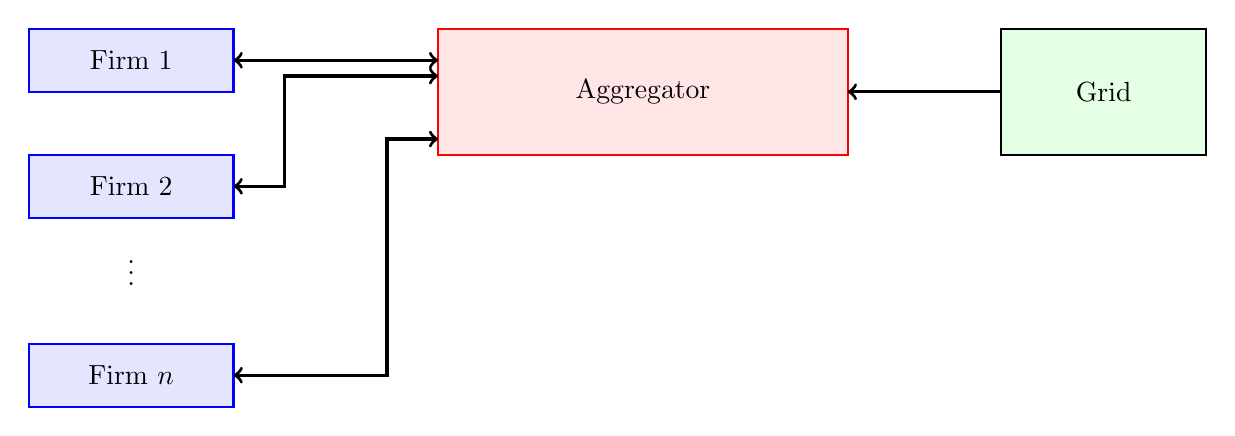
\begin{tikzpicture}[xscale=0.65, yscale=0.4]
\draw [blue, fill=blue, fill opacity = 0.1, thick] (-2,0) rectangle (2,2);
\node [align=center] at (0,1) {Firm $n$};
\node [align=center] at (0,4.5) {$\vdots$};
\draw [draw= blue, fill=blue, fill opacity = 0.1, thick] (-2,6) rectangle (2,8);
\node [align=center] at (0,7) {Firm $2$};
\draw [draw= blue, fill=blue, fill opacity = 0.1, thick] (-2,10) rectangle (2,12);
\node [align=center] at (0,11) {Firm $1$};
\draw [red, fill=red, fill opacity = 0.1, thick] (6,8) rectangle (14,12);
\node [align=center] at (10,10) {Aggregator};
\draw [fill=green, fill opacity = 0.1, thick] (17,8) rectangle (21,12);
\node [align=center] at (19,10) {Grid};
\draw [<->,very thick] (2,11) -- (6,11); 
\draw [<->,very thick] (2,7) --  (3,7) -- (3,10.5) -- (6,10.5); 
\draw [<->,very thick] (2,1) --  (5,1) -- (5,8.5) -- (6,8.5); 
\draw [<-,very thick] (14,10) --  (17,10);
\end{tikzpicture}
\end{center}

\bdashlist \setlength{\itemsep}{-0.02in}
\item $n$ firms, facing time-of-use pricing
\item \blue{Ex: industrial park, campus, housing complex}
\item firm $k$ invests in storage $C_k$ for arbitrage
\item unused stored energy is traded with other firms
\item AGG manages trading \& power transfer
\item collective deficit is bought from Grid
\end{list}

%------------------------------------------------

\subsection*{ToU Pricing and Storage}
\begin{center}
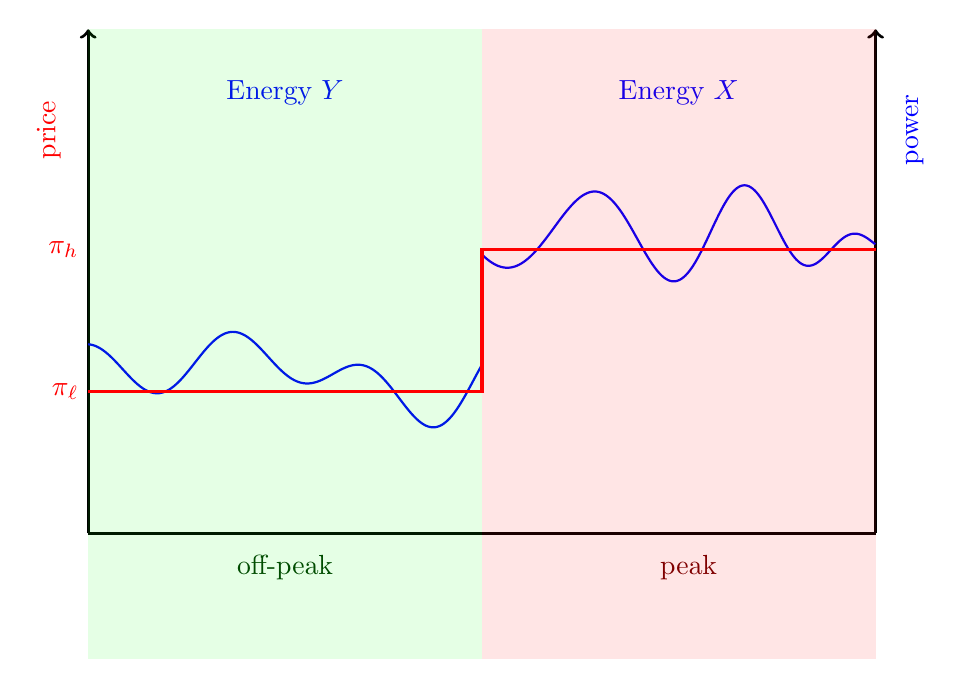
\begin{tikzpicture}[xscale=2.5, yscale = 1.6]
\draw[very thick] (0,0) -- coordinate (x axis mid) (4,0);
\node[align=right] at (2,-1) {};
\node[align=left,rotate=90,text=red] at (-0.2,3.2) {price};
\node[align=left,rotate=90,text=blue] at (4.2,3.2) {power};
\draw[very thick, ->] (0,0) -- coordinate (y axis mid) (0,4);
\draw[very thick, [->] (4,0) -- coordinate (y axis mid) (4,4);
%\foreach \y in {0,100}
%     		\draw (1pt,0.04*\y) -- (-3pt,0.04*\y)
%			node[anchor=east, align = left] {\y};	
%\foreach \x in {0,1}
%     		\draw (4*\x,1pt) -- (4*\x,-3pt)
%			node[anchor=north, align = right] {\x};				
\draw[blue, ultra thick, domain=0:2, samples=200, smooth, thick] plot (\x, {1.1+ 0.2*(cos(500*\x) + sin(100*\x^2) + exp(-0.5*\x) )});
\draw[blue, ultra thick, domain=2:4, samples=200, smooth, thick] plot (\x, {2.3 - 0.2*(sin(400*\x) + sin(90*\x^2) - exp(-0.3*\x) )});
\node[align=center, text=blue] at (1,3.5) {Energy $Y$};
\node[align=center, text=blue] at (3,3.5) {Energy $X$};
\draw [draw=none, fill=green, fill opacity = 0.1] (0,-1) rectangle (2,4);
\draw [draw=none, fill=red, fill opacity = .1] (2,-1) rectangle (4,4);
\draw [very thick,red] (0,1.125) --  (2,1.125) -- (2,2.25) -- (4,2.25);
\node[anchor=north, text=black!70!green] at (1,-0.1) {off-peak};
\node[anchor=east,text=red] at (0,2.25) {$\pi_h$};
\node[anchor=north, text=black!50!red] at (3.05,-0.1) {peak};
\node[anchor=east,text=red] at (0,1.125) {$\pi_\ell$};
%\node[anchor=west] at (0.3,3.5) {Pr $\{S \geq s\} = \rho$};
\end{tikzpicture}
\end{center}

\bdashlist
\item random consumption $X,Y$
\item \red{$F(x) =$ CDF of $X$}
\item \blue{value of storage: firm can move some purchase from peak to  off-peak}
    % charge in off-peak, discharge in peak
\end{list}

\section*{Consumption Model}
\begin{itemize}
\item \blue{Energy demand for firm $k$ is random}
\blist 
\item \red{$X_k$ in peak period, CDF $F_k (\cdot)$}
\item $Y_k$ in off peak period
\end{list}
\item \blue{Collective peak period demand}
\red{\[ X_c = \sum_k X_k, \ \text{ CDF } F_c (\cdot)
\]}
%\item Capital cost of storage
%\blist 
%\item amortized per day over lifetime of battery
%\item $\pi_s$ = price per day per KWh
%%\item today $\pi_s \approx 20$ cents, but falling fast
%\end{list}
%\item Time-of-use pricing
%\blist
%\item $\pi_h$ during peak period
%\item $\pi_\ell$ during off-peak
%\item difference $\pi_\delta = \pi_h - \pi_\ell$
%%\item need $\pi_\delta > \pi_s$ to justify storage investment for arbitrage alone
%%\item PG\&E A6 tariff ... $\pi_\delta \approx 25$ cents,
%%\item rarely happens today, but tomorrow $\pi_s$ will fall ...
%\end{list}

\end{itemize}


%%%%%%%%%%%%%%%%%%%%%%%%%%%%%%%%%
%%%%%%%%%%%%%%%%%%%%%%%%%%%%%%%%%

\section*{Prices and Arbitrage}

\blue{\begin{tabular}{r|l}
\quad $\pi_s$ & capital cost of storage \\
& amortized per day over battery lifetime \\[0.1in]
$\pi_h$ & peak-period price \\
$\pi_\ell$ & off-peak price \\
$\pi_\delta$ & difference $\pi_h - \pi_\ell$
\end{tabular}}

\begin{itemize}
\item Comments
\bdashlist
\item today $\pi_s \approx 20$ cents, but falling fast
\item need $\pi_\delta > \pi_s$ to justify storage investment for arbitrage alone
\item rarely happens today, but many more opportunities tomorrow  ...
\item ex: 
PG\&E A6 tariff ... $\pi_\delta \approx 25$ cents  $ > \pi_s = 20$ cents
\end{list}

\item \blue{Arbitrage constant 
\[ \quad \gamma = \frac{\pi_\delta - \pi_s}{\pi_\delta}  \quad \quad \gamma \in [0, 1] \]}
\end{itemize}


%%%%%%%%%%%%%%%%%%%%%%%%%%%%%%%%%
%%%%%%%%%%%%%%%%%%%%%%%%%%%%%%%%%

\section*{Assumptions}

\barablist
\item \blue{Firms are price-takers for ToU tariff ...} \\
consumption is not large enough to influence $\pi_h, \pi_\ell$
\item \blue{Demand is inelastic ... } \\
savings from using storage do not affect statistics of $X_k, Y_k$
\item \blue{Lossless storage, inverters are perfectly efficient} (temporary) 
\item \blue{Simultaneously decision making} (temporary) 
\end{list}


%%%%%%%%%%%%%%%%%%%%%%%%%%%%%%%%%
%%%%%%%%%%%%%%%%%%%%%%%%%%%%%%%%%

\section*{No Sharing: Firm's Decision}

\begin{itemize}
\item \blue{Daily cost components for firm $k$}

\begin{tabular}{c|l}
$\pi_{s} C_{k}$ & amortized cost for storage \\
$\pi_{h} (X_{k} - C_{k})_{+}$ & peak:  use storage first, buy deficit from grid \\
$ \pi_{\ell} \min\{C_{k}, X_{k}\}$ & off-peak: recharge storage
\end{tabular}
%
%\begin{list}{$-$}{}
%\item Amortized cost for storage: $\pi_{s} C_{k}$
%\item use storage first, buy deficit from grid $\pi_{h} (X_{k} - C_{k})_{+}$
%\item Recharge storage during off-peak: $ \pi_{l} \min\{C_{k}, X_{k}\}$
%\end{list}
\item \blue{Expected cost}
\begin{equation*}
J_{k}(C_{k}) = \pi_{s} C_{k} + \mathbb{E}\left[\pi_{h} (X_{k} - C_{k})_{+} + \pi_{\ell} \min\{C_{k}, X_{k}\}  \right]
\end{equation*}
%\[J_{k}(C_{k}) = \pi_{s} C_{k} + \mathbb{E}\left[\pi_{h} (X_{k} - C_{k})_{+} + \pi_{l} \min\{C_{k}, X_{k}\}  \right]\] 
\vspace{-0.5cm}
\end{itemize}

\noindent \textbf{Theorem 1: }
\red{Stand alone firm Optimal storage investment} 
\begin{equation}\nonumber
 C^{*}_{k} = \arg  min_{C_{k}} J_{k}(C_{k})  =   F^{-1}_{k}(\gamma) \quad \gamma = (\pi_{\delta} - \pi_{s})/\pi_{\delta}
\end{equation}



%%%%%%%%%%%%%%%%%%%%%%%%%%%%%%%%%
%%%%%%%%%%%%%%%%%%%%%%%%%%%%%%%%%

\begin{itemize}
\item \red{Without sharing, firms make sub-optimal investment choices:}
\bdashlist
\item \blue{firms may over-invest in storage! \\
not exploiting other firms storage, if $\gamma$ is large 
\item or under-invest! \\
not taking into account of profit opportunities, if $\gamma$ is small}
\end{list}
\item More precisely:
\bdashlist
\item optimal storage investment for collective 
\[ C^{*}_{c} =  F_c^{-1}(\gamma), \quad   \sum_{k} X_{k} = X_c \sim F_c(\cdot) \]
\item total optimal investment for stand-alone firms $\sum_k C_k^\ast$
\item under-investment $C^{*}_{c} > \sum_{k} C^{*}_{k}$ \\
 over-investment: $C^{*}_{c} < \sum_{k} C^{*}_{k}$
\end{list}
\end{itemize} 

%%%%%%%%%%%%%%%%%%%%%%%%%%%%%%%%%
%%%%%%%%%%%%%%%%%%%%%%%%%%%%%%%%%

\section*{Example: Two Firms}


\bdashlist
\item $X_{1}, X_{2} \sim U[0, 1]$, independent
\item individual investments: $C^{*}_{k} = F^{-1}_{k}(\gamma) = \gamma$ \\
\item collective investment: $C_c^\ast = F^{-1}_{c}(\gamma)$ where $X_c = X_1 + X_2$
%\[ F_X(x) = \left\{ \begin{array}{cl} 0.5 x^2  & \text{ if } x \in [0,1] \\
%1 - 0.5(x -2)^2 & \text{ if } x \in [1,2] \end{array} \right. 
%\]
%\item optimal investment for collective 
\[ C^{*}_{c} =  \left\{ \begin{array}{cl}
\sqrt{2 \gamma} & \text{ if } \gamma \in [0, 0.5]   \\ 2 + \sqrt{2 - 2\gamma} & \text{ if } \gamma \in [0.5,1]   
\end{array} \right. \]
\end{list}

%\captionsetup{justification=centering}
\begin{center}
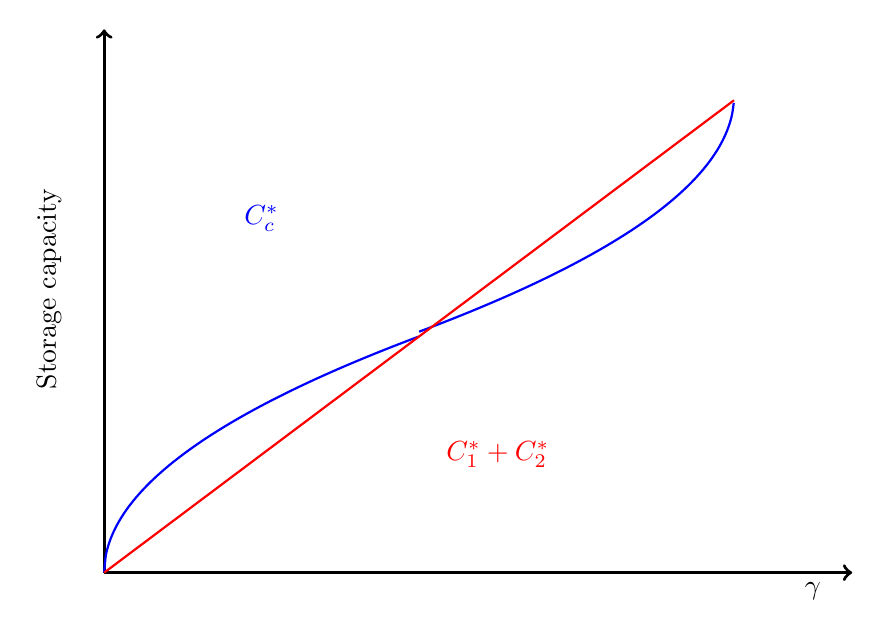
\begin{tikzpicture}[xscale=2, yscale = 3]
\draw[very thick,->] (0,0) -- coordinate (x axis mid) (4.75,0);
\draw[very thick, ->] (0,0) -- coordinate (y axis mid) (0,2.3);
\node[align=left,rotate=90,text=black] at (-0.35,1.2) {Storage capacity};
\node[anchor=north,text=black] at (4.5,0) {$\gamma$};
\draw[blue, ultra thick, domain=0:2, samples=200, smooth, thick] plot (\x, {  sqrt(0.5*\x)  });
\draw[blue, ultra thick, domain=2:4, samples=200, smooth, thick] plot (\x, {  2.02 - sqrt(2 - 0.5*\x)  });
\draw[red, ultra thick, domain=0:4, samples=200, smooth, thick] plot (\x, {  0.5 *\x  });
\node[align=center, text=blue] at (1,1.5) {$C_c^\ast$};
\node[align=center, text=red] at (2.5,0.5) {$C_1^\ast + C_2^\ast$};
%\node[anchor=north, text=black!70!green] at (1,-0.1) {off-peak};
%\node[anchor=east,text=red] at (0,2.25) {$\pi_h$};
%\node[anchor=north, text=black!50!red] at (3.05,-0.1) {peak};
%\node[anchor=east,text=red] at (0,1.125) {$\pi_\ell$};
%\node[anchor=west] at (0.3,3.5) {Pr $\{S \geq s\} = \rho$};
\end{tikzpicture}
\end{center}
%\caption{Under- and over-investment.}% \label{fig:example}


%%%%%%%%%%%%%%%%%%%%%%%%%%%%%%%%%
%%%%%%%%%%%%%%%%%%%%%%%%%%%%%%%%%

\section*{Sharing Storage}

\begin{itemize}
\item Firm $k$  has surplus energy in storage $(C_k - X_k)^+$
\bdashlist
\item can be sold to other firms who might have a deficit
\item willing to sell at acquisition price $\pi_\ell$
\end{list}
\item \blue{Supply and demand}
\bdashlist
\item collective surplus: $S = \sum_k (C_k - X_k)^+ $
\item collective deficit: $D = \sum_k (X_k - C_k)^+ $
\end{list} 
\item \red{Spot market for sharing storage} 
\bdashlist
\item if $S>D$ firms with surplus compete \\  energy trades at the price floor $\pi_\ell$
\item if $S<D$ firms with deficit must buy some energy from grid \\ 
 energy trades at price ceiling $\pi_h$
\end{list}
\end{itemize}

%%%%%%%%%%%%%%%%%%%%%%%%%%%%%%%%%
%%%%%%%%%%%%%%%%%%%%%%%%%%%%%%%%%


\section*{Spot Market}

\begin{itemize}
%\item Supply and demand
%\begin{list}{$-$}{}
%\item Surplus charge: $S = \sum_k (C_k - X_k)^+ $
%\item Deficit charge: $D = \sum_k (X_k - C_k)^+ $
%\end{list} 
\item \red{Market clearing price
\[\pi_{eq} = \left\{ \begin{array}{cl} \pi_l & \text{ if } S > D \\ \pi_h & \text{ if } S < D  \end{array} \right.\] }
\item \blue{Random, depends on daily market condns}
\end{itemize}

\begin{figure}
%\captionsetup{justification=centering}
\centering
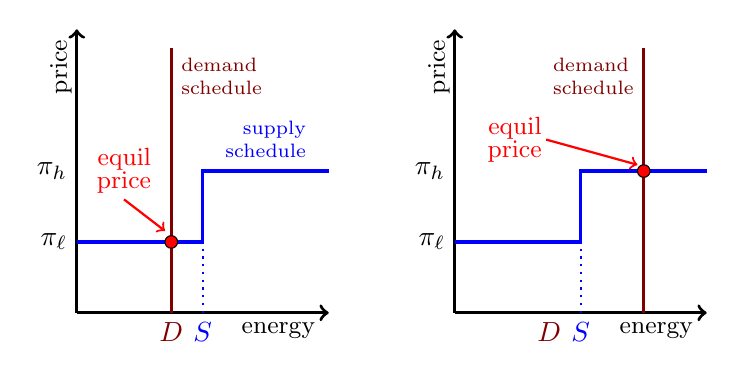
\begin{tikzpicture}[xscale=0.8, yscale = 0.8]
\begin{scope}
\draw[very thick,->] (0,0) -- coordinate (x axis mid) (4,0);
\node[align=left,rotate=90,text=black] at (-0.25,3.9) {\small price};
\node[anchor=north,text=black] at (3.2,0) {\small energy};
\node[anchor=north,text=black!50!red] at (1.5,0) {$D$};
\node[anchor=north,text=blue] at (2,0) {$S$};
\draw[very thick, ->] (0,0) -- coordinate (y axis mid) (0,4.5);		
\node[align=right, text=blue] at (3,2.75) {\scriptsize supply \\[-0.05in] \scriptsize schedule};
\node[align=left, text=black!50!red] at (2.3,3.75) {\scriptsize demand \\[-0.05in] \scriptsize schedule};
\node[align=right, text=red] at (0.75,2.25) {\small equil \\[-0.05in] \small price};
\draw [thick,red, ->] (.75,1.8) --  (1.4,1.3);
\draw [very thick,blue] (0,1.125) --  (2,1.125) -- (2,2.25) -- (4,2.25);
\draw [thick,blue, dotted] (2,0) --  (2,1.125);
\draw [very thick, black!50!red] (1.5, 0) -- (1.5,4.2);
\draw [fill=red] (1.5,1.125) circle [radius=0.1];
\node[anchor=east,text=black] at (0,2.25) {$\pi_h$};
\node[anchor=east,text=black] at (0,1.125) {$\pi_\ell$};
\end{scope}
\begin{scope}[shift={(6,0)}]
\draw[very thick,->] (0,0) -- coordinate (x axis mid) (4,0);
\node[align=left,rotate=90,text=black] at (-0.25,3.9) {\small price};
\node[anchor=north,text=black] at (3.2,0) {\small energy};
\node[anchor=north,text=black!50!red] at (1.5,0) {$D$};
\node[anchor=north,text=blue] at (2,0) {$S$};
\draw[very thick, ->] (0,0) -- coordinate (y axis mid) (0,4.5);		
%\node[align=right, text=blue] at (3,2.75) {\small supply \\[-0.05in] \small schedule};
\node[align=left, text=black!50!red] at (2.2,3.75) {\scriptsize demand \\[-0.05in] \scriptsize schedule};
\node[align=right, text=red] at (0.95,2.75) {\small equil \\[-0.05in] \small price};
\draw [thick,red, ->] (1.45,2.75) --  (2.9,2.35);
\draw [very thick,blue] (0,1.125) --  (2,1.125) -- (2,2.25) -- (4,2.25);
\draw [thick,blue, dotted] (2,0) --  (2,1.125);
\draw [very thick, black!50!red] (3, 0) -- (3,4.2);
\draw [fill=red] (3,2.25) circle [radius=0.1];
\node[anchor=east,text=black] at (0,2.25) {$\pi_h$};
\node[anchor=east,text=black] at (0,1.125) {$\pi_\ell$};
\end{scope}
\end{tikzpicture}
%\caption{Equilibrium Price: (a) left panel $S>D$, (b) right panel $S < D$. } \label{fig:equil}
\end{figure} 

%\[ D - S =  \sum_k (X_k - C_k)^+  - \sum_k (C_k - X_k)^+ = \sum_k (X_k - C_k) \]


%%%%%%%%%%%%%%%%%%%%%%%%%%%%%%%%%
%%%%%%%%%%%%%%%%%%%%%%%%%%%%%%%%%

\section*{Firm's Decisions Under Sharing}
\begin{itemize}
\item Expected cost for firm $k$
\[  J_k(C_k \mid C_{-k}) =  \pi_s C_k + \pi_{l} C_k + \mathbb{E}[ \pi_{eq} (X_k - C_k)^{+} - \pi_{eq} (C_{k} - X_{k})^{+}]\]
\item \red{Storage Sharing Game}
\bdashlist
\item players: $n$ firms, decisions: storage investments $C_{k}$
\item optimal investment $C^{\ast}_{k}$ depends on the investment of other firms 
\end{list}

\item  Expected cost for collection of firms $\sum_k J_k$
\bdashlist
\item like a single firm without sharing
\end{list}
\item \red{Social Planner's Problem}
\[ \min_{C_c} J_a(C_c) \quad \quad \text{solution: } \ \ C_c^* = F_c^{-1}(\gamma) \]
\end{itemize}

\noindent \textbf{Theorem 2:}
\balphlist
\item Storage Sharing Game admits unique Nash Equilibrium
\item Optimal storage investments:
\[ C^{\ast}_k = \mathbb{E}[X_k \mid X_c=C_c],~~ \textnormal{where}~C_c = \sum_{k} C^{\ast}_{k},~ F(C_c) = \gamma  \] 
\vspace*{-0.2in}

%\item expected clearing price $\Eset \left[ \pi_{eq} \right] = \pi_s$
\item Nash equilibrium supports the social welfare
%\item investment decisions of each firm is individually rational 
\item Equilibrium is coalitional stable -- no subset of firms will defect
\item Nash equilibrium is also the (unique) cooperative game equilibrium
\end{list}

%\begin{theorem}
%\balphlist
%\item Nash equilibrium supports the social welfare
%%\item investment decisions of each firm is individually rational 
%\item equilibrium is coalitional stable -- no subset of firms will defect
%\item Nash equilibrium is also the (unique) cooperative game equilibrium
%%\item no pure storage play
%%\[ X_k \equiv 0 \ \implies C_k^\ast = 0 \]
%\end{list}
%\end{theorem}



%%%%%%%%%%%%%%%%%%%%%%%%%%%%%%%%%
%%%%%%%%%%%%%%%%%%%%%%%%%%%%%%%%%

\section*{Lossy Storage}

\begin{itemize}
\item More realistic storage model
\bdashlist
\item charging efficiency $\eta_i \approx 0.95$
\item discharging efficiency $\eta_o \approx 0.95$
\item daily leakage $\epsilon$ (holding cost)
\end{list}
\item \red{Storage parameters modify arbitrage constant}
\end{itemize}

\noindent \textbf{Theorem 3:}
Optimal investment of collective is
\[ C_a^\ast = \frac{1}{\eta_o} \cdot F_a^{-1} (\gamma), \quad \text{where    } 
\gamma = \frac{\pi_h \eta_o \eta_i - \pi_\ell - \eta_i \pi_s   }{ \pi_h \eta_o \eta_i - \pi_\ell ( 1 - \epsilon) } 
\]


%%%%%%%%%%%%%%%%%%%%%%%%%%%%%%%%%
%%%%%%%%%%%%%%%%%%%%%%%%%%%%%%%%%

\section*{Sequential Investment Decisions}

\begin{itemize}
\item Collective of $n$ firms have optimally invested $C^n$ in storage
\item \red{Now firm $F_{n+1}$ want to join the club}
\item Optimal investment of new collective is $C^{n+1}$ 
\end{itemize}

\noindent \textbf{Theorem 4:}
Optimal storage investment is {\sl extensive}, i.e. increases as new firms join
\[ C^{n+1} \geq C^n \]

\begin{itemize}
\item \blue{Who benefits?}
\bdashlist
\item  $F_{n+1}$ is better off by joining 
\item collective is bettor off when $F_{n+1}$ joins 
\item \red{but do firms in the collective individually benefit? don't know}
% installed and managed by aggregator
\end{list}
\end{itemize}

%%%%%%%%%%%%%%%%%%%%%%%%%%%%%%%%%
%%%%%%%%%%%%%%%%%%%%%%%%%%%%%%%%%

\section*{Joining the Club}

\begin{itemize}
\item \blue{Optimal ownership redistributes when $F_{n+1}$ joins}
\[ C^n = (\alpha_1, \cdots, \alpha_n) \ \ \rightarrow \ \ C^{n+1} = (\beta_1,  \cdots, \beta_n, \beta_{n+1}) \] 
\item \blue{Actions}
\bdashlist
%\item buys $\beta_{n+1}$ units of storage, owns revenue stream
\item new firm $F_{n+1}$ pays the collective $\pi_s \beta_{n+1}$
\item receives rights and revenue stream for $\beta_{n+1}$ units of storage
\item collective invests in $C^{n+1} - C^{n}$ additional storage 
\item internal exchange of money and storage ownership within collective
\end{list}
\end{itemize}

%%%%%%%%%%%%%%%%%%%%%%%%%%%%%%%%%
%%%%%%%%%%%%%%%%%%%%%%%%%%%%%%%%%


\section*{Market Implementation}

\noindent \textbf{Theorem}
No pure storage play:
\[ X_k \equiv 0 \ \implies C_k^\ast = 0 \]
Therefore AGG is in a neutral financial position



\begin{itemize}
\item \blue{Privacy and market clearing}
\bdashlist
\item to determine its investment $C_k^\ast$, firm $k$ need knowledge of collective investment and statistics
\item informed by neutral AGG
\item AGG determines clearing price $\pi_{eq}$ each day
\end{list}

\item \blue{Other market choices?}
\bdashlist
\item bulletin board for P2P bilateral trades
\item matching market hosted by AGG
\end{list}
\end{itemize}


\end{multicols}
\end{document}